% !TeX spellcheck = en_US
\chapter{The Paretian preference}
\label{ch:paretian}

We now consider a more complex decision framework: still a single decision maker and a single scenario, but the preference relation is no longer a weak order described by a consistent value (or cost) function.

We assume: 
\begin{itemize}
	\item A preference relation $\Pi$ that is no longer a weak order
	
	\item A certain environment $|\Omega| = 1 \implies f(x, \bar \omega)$ reduces to $f(x)$
	
	\item A single decision-maker: $|D| = 1 \implies \Pi_d$ reduces to $\Pi$
\end{itemize}
If $\Pi$ is a preorder, we at least have nondominated solutions $X^\circ$ but possibly incomparable with each other. 

We want to make assumption on the structure of the preference relation (different assumptions will lead to different models); the first model proposed in history is the one proposed by \href{https://en.wikipedia.org/wiki/Vilfredo_Pareto}{\texttt{Vilfredo Pareto}}. \\

\begin{definition}
	We denote as \textbf{Paretian preference} the relation
	$$ \Pi = \left\{(f, f') \mid f_l \leq f_l' \text{ for each } l \in \{1, \dots, p\}\right\} $$
	that is
	$$ f \leq f' \Leftrightarrow f_l \leq f_l' \text{ for each } l \in \{1, \dots, p\} $$
\end{definition}

This assumes that each indicator represents a cost (easily extendable to the benefit and mixed cases). 

This models only allows to compare impacts with elements that dominate each other all in the same orientation; this \textbf{incomparable indicators assumption}, meaning that the decision-maker is unable to compare two impacts when different indicators give opposite suggestions. This can make the model unrealistic.

This model can seem not very useful to make an actual choice, as it ends with proposing several incomparable solutions, but in practice it's a useful starting point to further refine the preference relation.

\section{Properties of the Paretian preference}
\label{sec:paretoproperties}

\begin{theo}
	The Paretian preference relation is a partial order (reflexivity, antisymmetry and transitivity).
\end{theo}

\begin{proof}
	In fact, it is
	\begin{itemize}
		\item Reflexive: $f \wpref{} f$, for all $f \in F$
		\begin{align*}
			&f_l = f_l, \ \forall l \in \{1, \dots, p\}  \\
			\implies & f_l \leq f_l, \ \forall l \in \{1, \dots, p\}  \\
			\implies & f \wpref{} f
		\end{align*}
		
		\item Transitive: $f \wpref{} f'$ and $f' \wpref{} f'' \implies f \wpref{} f''$ for all $f, f', f'' \in F$
		$$
		\begin{cases}
			f \wpref{} f' \\
			f' \wpref{} f''
		\end{cases}
		\implies \begin{cases}
			f_l \leq f_l' & \forall l \in \{1, \dots, p\} \\
			f_l' \leq f_l'' & \forall l \in \{1, \dots, p\}
		\end{cases}
		\implies 
		$$
		$$ \implies f_l \leq f_l'', \ \forall l \in \{1, \dots, p\} \implies f \wpref{} f'' $$
		
		\item Antisymmetric: $f \wpref{} f'$ and $f' \wpref{} f \implies f = f'$ for all $f, f' \in F$
		$$ 
		\begin{cases}
			f \wpref{} f' \\
			f' \wpref{} f
		\end{cases}
		\implies \begin{cases}
			f_l \leq f_l' & \forall l \in \{1, \dots, p\} \\
			f_l' \leq f_l & \forall l \in \{1, \dots, p\}
		\end{cases}\implies 
		$$
		$$ \implies f_l = f_l', \ \forall l \in \{1, \dots, p\} \implies f = f' $$
	\end{itemize}
\end{proof}

This can appear as trivial, bu the translation from the relation on impacts ($\wpref{}$) to the relation of indicators ($\leq$) is allowed only by Pareto's definition.

In general, the Paretial preference relation is \textbf{not complete}.

\section{Paretian dominance}
\label{sec:paretiandom}

We can reformulate the concept of domination: a solution dominates another if and only if the impact of the former is strictly preferred to the impact of the latter. The preference is strict to avoid rejecting all indifferent solutions (they should not dominate each other).

In the Pareto case, dominance is expressed as follows
$$ x' \prec x \Leftrightarrow f(x') \prec f(x) \Leftrightarrow \begin{cases}
	f_l (x') \leq f_l (x), \ \forall l \in \{1, \dots, p \} \\
	\exists \bar l \in \{1, \dots, p\} : f_{\bar l} (x') < f_{\bar l} (x)
\end{cases}$$

allowing to split feasible solutions in two groups, one of which can be rejected in every reasonable decision.\\

\begin{definition}
	We denote as \textbf{dominated solution} every feasible solution $x \in X$ that admits another solution $x' \in X$ which dominates it: 
	$$ 
	\exists x' \in X, \ \bar l \in \{1, \dots , p \} : \begin{cases}
		f_l (x') \leq f_(x), \ \forall l \in \{1, \dots, p\} \\
		f_{\bar l} (x') < f_{\bar l} (x)
	\end{cases}
	$$
\end{definition}

\begin{definition}
	We denote as \textbf{Paretian solution} every feasible solution $x \in X$ such that no other solution $x'$ dominates it
	$$ \forall x' \in X, \ \exists \bar l \in \{1, \dots, p\} : f_{\bar l} (x) < f_{\bar l} (x') \text{ or } f(x') = f(x) $$
\end{definition}

\begin{definition}
	We denote as \textbf{Paretian region} $X^\circ$ the set of all paretian solutions.
\end{definition}

Unless for infinite chains, $X^\circ$ is nonempty and contains reciprocally incomparable solutions (or indifferent solutions that have the same impact). The aim is to enumerate $X^\circ$ and then ask the decision-maker.

The Paretian region corresponds to the set of globally optimal points in Mathematical Programming, with two differences, due to the incompleteness of the Paretian preference: 
\begin{enumerate}
	\item the Paretian solutions are not preferable to all other solutions, whereas the globally optimal points are
	
	\item the Paretian solutions are not reciprocally indifferent, whereas the globally optimal points are
\end{enumerate}

This means that is not enough to find a single globally optimal point and ignore the others as is Mathematical Programming, in the Paretian case it's appropriate to find all Paretian solutions.

\section{Identification of the Paretian region}
\label{sec:identifyparetianregion}

The fundamental problem now is how to determine the Paretian region. We'll look at different ways to obtain it which provide, in general, different results, due to the fact that they usually generate an underestimate (subset) or overestimate (superset) of $X^\circ$.

Some methods to enumerate the Paretian region:

\resizebox{\textwidth}{!}{
	\renewcommand{\arraystretch}{1.4}
	\begin{tabular}{L{3cm} | L{2cm} | L{4cm} | L{3.1cm}}
		\textbf{Method} & \textbf{Generality} & \textbf{Practical limits} & \textbf{Result provided} \\
		\hline
		definition & finite & slow for CO & exact \\
		
		inverse transformation & $p = 2$ & human intervention & exact \\
		
		KKT conditions & regular & solving a system & overestimate \\
		
		weighted sum & general & parametric problem (inefficient sampling) & underestimate (bad for large $p$) \\
		
		$\varepsilon$-constraint & general & parametric problem, usually NP-hard (inefficient sampling) & overestimate (refined by repetition) \\
	\end{tabular}
}

\subsection{Applying the definition}
\label{subsec:applyingdefinition}

In the finite case, $X^\circ$ can be found by pairwise comparisons, of course taking $\Theta\left(p|X|^2\right)$ time in the worst case. \textit{This can be huge in combinatorial problems, where $|X| \in \Theta\left(2^n\right)$}.

We can build the solution dominance graph, whose nodes correspond to solutions and whose arcs correspond to the dominance relation. The solutions are nodes with no outgoing arcs.

\section{Inverse transformation method}
\label{sec:invtransformation}

This method also consists in applying the definition, but can be used on continuous problems, provided that they can be graphically represented in the indicator space. In fact, the method consists in a graphical solution of the problem, and requires to:
\begin{itemize}
	\item Determine the inverse $\phi: F \rightarrow X$ of the transformation $f: X \rightarrow F$ (if not unique, compute all inverse functions)
	
	\item Build the image of $X$ in $F$ through the impact function $f(x)$ by drawing the constraints $g_j (x(f)) \leq 0$
	
	\item Find graphically the nondominated impact subset $F^\circ \subset F$, exploiting the property that these impacts have an empty lower left quadrant (human intervention, it's graphical)
	
	\item Find a parametric form $f^\circ (\alpha)$ to describe $F^\circ$
	
	\item Transform $F^\circ$ into $X^\circ$ through the inverse function $\phi(f^\circ(\alpha))$
\end{itemize}

Basically, compute the inverse function, apply $f$ to all $x \in X$, find graphically the nondominated impacts, find a parametric way to describe the set of nondominated impacts, transform them back using the inverse function.

\section{Karush-Kuhn-Tucker conditions}
\label{sec:kktcondforpareto}

The KKT conditions can be extended to Pareto preference by repeating the derivation with minor changes, obtaining a set $X^{KKT}$ that is generally larger than the Paretian region.

\subsubsection{Locally Paretian solutions}

\begin{definition}
	We denote as \textbf{locally Paretian solution} a feasible solution $x \in X$ that admits a neighborhood $\U_{x, \epsilon}$ in which no other solution dominates it
	$$ \exists \U_{x, \epsilon} : x' \not \prec x, \ \forall x' \in \U_{x, \epsilon} \cap X $$
\end{definition}

A Paretian solution is always locally Paretian, while the opposite doesn't always hold (similar to global and local optimum). Let $X^\ast$ denote the set of all locally Paretian points. \\

\begin{theo}
	If $X = \{x \in R^n \mid g_j (x) \leq 0 \text{ for } j =1, \dots, m\}$ with $f_l (\cdot), g_j(\cdot) \in C^1 (X)$ then 
	$$ X^\circ \subseteq X^\ast \subseteq X^{KKT}$$
	The KKT conditions are necessary for local paretianity.
\end{theo}

The figure below shows in white the set $F$ of impacts of a decision problem in the indicator space $\R^p$. To check whether an impact corresponds to a dominated or Paretian point is enough to verify that the lower left quadrant built from each point does not include any other points.
\begin{center}
	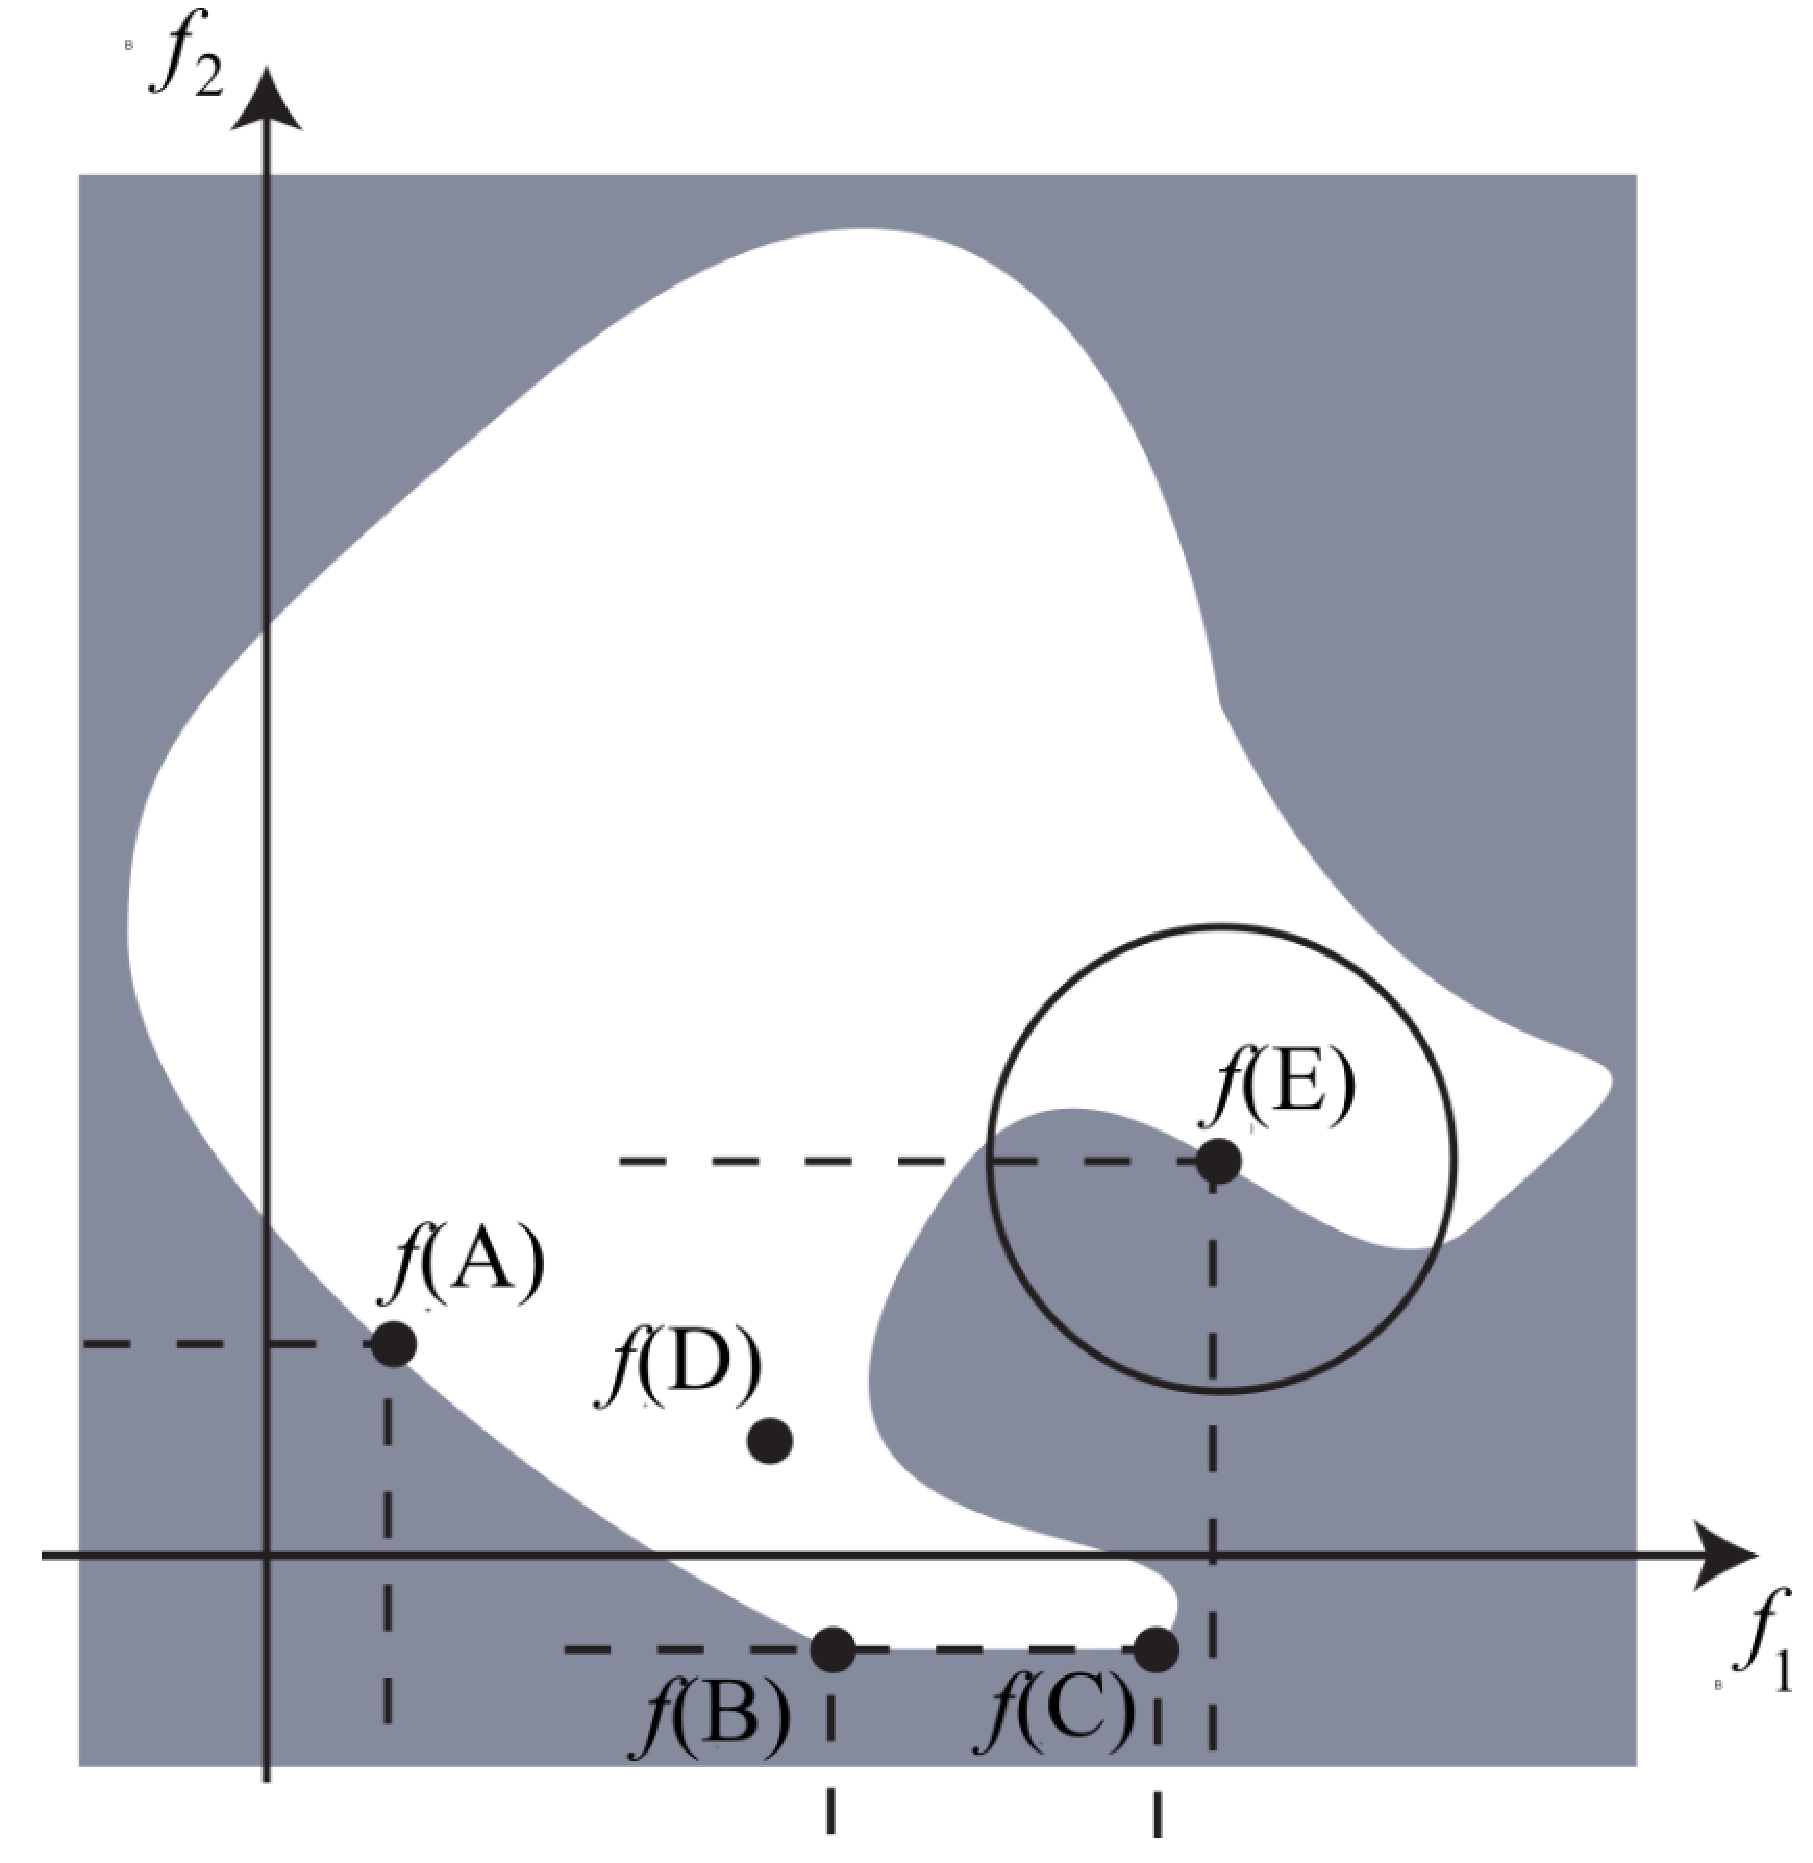
\includegraphics[width=0.5\columnwidth]{img/mcp/paretian/locpar}
\end{center}

We can see that
\begin{itemize}
	\item $D$ is dominated: there are impacts below and on the left of $f(D)$
	
	\item $A$ and $B$ are globally Paretian: their lower left quadrant is empty
	
	\item $E$ is locally Paretian: the quadrant is empty in a neighborhood
	
	\item $C$ is weakly Paretian: one indicator value is identical
\end{itemize}

If $X$ is discrete, all feasible solutions are isolated points, this means that, with a small enough $\epsilon$, every point can be locally Paretian with respect to $\U_{x, \epsilon}$. In the discrete case, once again, the overestimate given by the KKT conditions reduces to the whole set of feasible solutions.

\subsubsection{Sketch of the proof}

\paragraph{Definition} If a point $x$ is locally Paretian, all the arcs $\xi$ feasible in $x$ are nonimproving.

\paragraph{Nonimproving condition} We replace all indicators with their first-order approximation. The directions in which indicator $f_l$ is nonimproving satisfy condition $(\nabla f_l (x))^T p \geq 0$.\\

\begin{theo}
	If $\xi (\alpha)$ is a feasible arc in $x$ and $\nabla f_l (x)^T p < 0$ for all $l \in P$, then $x$ is not a locally Paretian point.
\end{theo}

It is a sufficient condition to prove that $\xi(\alpha)$ is an improving arc for $f(\cdot)$ in $x$, and therefore to filter $x$ out of the candidate set $X^{KKT}$.

Notice that improving all indicators is not necessary for strict dominance: weakly Paretian points are dominated, but some indicators can't improve. Therefore, weakly Paretian points satisfy the KKT conditions.

\paragraph{Feasibility condition} Feasibility is treated the same way as in Mathematical Programming: 
\begin{itemize}
	\item nonregular points are candidate
	
	\item a regular point $x$ is feasible if and only if
	$$ \nabla g_j(x)^T p \leq 0, \ \forall j \in J_a (x) $$
\end{itemize}

\paragraph{First geometric interpretation} Combining feasibility and nonimprovement implies that, if a point $\tilde x$is regular and locally Paretian and $p$ is a vector such that $(\nabla g_j)^Tp < 0$ for all constraints active in $\tilde x$ (vector tangent to a feasible arc), then there exists at least one indicator $f_l$ such that $(\nabla f_l)^T p \geq 0$ (an indicator that does not strictly improve along the arc).

Remembering the definition of feasible and improving cones (see \ref{subsec:firstgeometricinterpretation}), if a regular point is locally Paretian, then its feasible cone and improving cone do not intersect.
$$ x \in X^\ast \implies C_{feas} (x) \cap C_{impr} (x) = \emptyset $$

\paragraph{Farkas' lemma} The application of Farkas' lemma is somewhat more complicated than in Mathematical Programming, because there is no longer a single vector on one hand and a cone on the other. The workaround is to introduce an auxiliary vector and apply the lemma twice: to the auxiliary vector and the feasible cone and to the opposite of the auxiliary vector and the improving cone.

The existence of two cones which do not intersect is equivalent to the existence of hyperplane separating them that has two opposite orthogonal vectors: 
\begin{itemize}
	\item Vector $\gamma$ is on the opposite side of all $p \in C_{feas}$
	$$ p^T \gamma \leq 0, \ \forall p : p^T \nabla g_j (x) \leq 0, \ \forall j \in J_a (x) $$
	
	\item Vector $- \gamma$ is on the opposite side of all $p \in C_{impr}$
	$$ p^t (- \gamma) \leq 0, \ \forall p : \nabla f_l (x)^T (-p) < 0, \ \forall l \in P $$
\end{itemize}
Now we can apply Farkas' lemma to both expressions, obtaining that
\begin{itemize}
	\item Vector $\gamma$ falls in the cone of the gradients of the active constraints
	$$ \exists \mu_j \geq 0 : \gamma = \sum_{j \in J_a (x)} \mu_j \nabla g_j (x) $$
	
	\item Vector $- \gamma$ falls in the cone of the gradients of the objectives
	$$ \exists w_l \geq 0: - \gamma = \sum_{l \in P} w_l \nabla f_l (x) $$
\end{itemize}
Summing the two equations, one obtains the thesis:
$$ \exists \mu_j\geq 0, \ w_l \geq 0 : \sum_{l \in P} w_l \nabla f_l (x) + \sum_{j \in J_a (x)} \mu_j\nabla g_j (x) = 0$$
These are the KKT conditions for the Paretian case.

\paragraph{Standard form of the KKT-conditions} As in Mathematical Programming, the nonactive constraints can be reintroduces by imposing that their multipliers be zero, thanks to the complementarity conditions $\mu_j g_j (x) = 0$, and the equality constraints can be treated without explicitly replacing them with pairs of inequalities through the use of free multipliers.

Notice that, for any solution $(x, w, \mu)$, also $(x, \alpha w, \alpha \mu)$ is a solution, that provides the same candidate point $x$ (for any $\alpha > 0$). In other words, the multipliers have a degree of freedom that does not affect the solution. 

To remove this freedom we impose a normalization condition. Usually this is done by dividing all multipliers by $\sum_{l = 1}^p w_l$ so that
$$ \sum_{l = 1}^p w_l = 1$$

This requires to prove that $\sum_l w_l > 0$, but this is true because the gradients of the active constraints are linearly independent in all regular points and therefore $\sum_j \mu_j \nabla g_j \neq 0$.

\paragraph{Equation balance} The KKT condition system has $n+p+m$ variables: 
\begin{itemize}
	\item $n$ variables for vector $x$
	
	\item $p$ variables for vector $w$
	
	\item $m$ variables for vector $\mu$
\end{itemize}
and $n+1+m$ equalities
\begin{itemize}
	\item $n$ equations for the KKT conditions
	
	\item $1$ equation for the normalization condition
	
	\item $m$ equations for the complementarity conditions
\end{itemize}

In general, it will have $\infty^{p-1}$ solutions describing a hypersurface.

% End L10, notes p174

\section{The weighted-sum method}
\label{sec:weightedsum}

The weighted-sum method consists in building a linear combination of the indicators and minimizing it. The result is a sufficient condition for a point to be globally Paretian. \\

\begin{theo}
	Let $z(x) = \sum_{l = 1}^p w_l f_l (x)$ be a convex combination of the indicators, with coefficients $w_l > 0$ for $l \in \{1, \dots, p\}$ and $\sum_{l = 1}^p w_l = 1$. If $x^\circ$ is a globally optimal point for problem 
	$$ \min_{x \in X} z(x) \sum_{l = 1}^p w_l f_l (x) $$
	then $x^\circ$ is a globally Paretian point with respect to the impact $f(x)$.
\end{theo}
\begin{proof}
	The proof is by contradiction. If $x^\circ$ were not a Paretian point, by definition there should exist another point $x' \in X$ such that $x' \prec x^\circ$, that is $f_l (x') \leq f_l(x^\circ)$ for each $l \in \{1, \dots, p\}$, and an index $\bar l$ such that $f_{\bar l} (x') < f_{\bar l} (x^\circ)$. But this would imply
	$$ 
	\begin{cases}
		w_l f_l (x') & \leq w_l f_ (x^\circ), \ \forall l \in \{1, \dots, p\} \setminus \{\bar l\} \\
		w_{\bar l} f_{\bar l} (x') & < w_{\bar l} f_{\bar l} (x^\circ)
	\end{cases}
	$$
	Notice that the second property holds only if $w_{\bar l}$ is strictly positive. Summing the $p$ inequalities, one obtains
	$$ \sum_{l = 1}^p w_l f_l (x') < \sum_{l = 1}^p w_l f_l (x^\circ) \implies z(x') < z(x^\circ) $$
	and therefore $x^\circ$ cannot be a globally optimum point for $z(x)$. From the contradiction the thesis follows.\\
\end{proof}

The combination is convex, but the weights $w_l$ are strictly positive. If weights equal to zero were allowed, the proof would not hold, because weakly Paretian solutions satisfy the condition, even if dominated.

Let $W = \left\{w \in \R^p \mid w_l > 0, \ \forall l \in P, \ \sum_{l \in P} w_l = 1 \right\}$ be the weight space. \\

\begin{definition}
	Given a Paretian solution $x^\circ \in X^\circ$, we denote as \textbf{support} of $x^\circ$ the set $\supp(x^\circ) \subset W$ of weight vectors $w$ such that $x^\circ$ is a globally optimal point for the problem $\min_{x \in X} \sum_{l = 1}^p w_l f_l (x)$.
\end{definition}

Continuous problems usually have $\infty^{p-1}$ Paretian solutions and $\infty^{p-1}$ weight vectors: the support of a Paretian solution often includes a single vector. 

Finite or combinatorial problems have a finite number of solutions: the support of a Paretian solution often is a region in the weight space. 

In general, however, unsupported solutions exist. The weighted-sum method finds only supported solutions. \\

\begin{definition}
	We denote as \textbf{supported solution} a Paretian solution $x^\circ \in X^\circ$ whose support is nonempty: $\supp (x^\circ) \neq \emptyset$.
\end{definition}

The assumptions of the weighted-sum method are stricter than the KKT conditions (solution $x^\circ$ be a globally optimal point instead of candidate locally optimal ones, and strictly positive coefficients $w_l$ are imposed), making them sufficient to guarantee a point being Paretian, instead of only necessary. Consequently, this yields $X^{WS} \subseteq X^\circ$, subset instead of superset.

\paragraph{Combinatorial Example} Given a complete graph of three vertices and two cost function, find the minimum spanning tree
\begin{center}
	\begin{tabular}{c | c c c}
		$f(x)$ & $(1,2)$ & $(1,3)$ & $(2,3)$ \\
		\hline
		$f_1$ & 1 & 3 & 6 \\
		$f_2$ &13 & 10 & 8 
	\end{tabular}
\end{center}
The KKT-conditions are useless in this case, since it's a discrete problem, and therefore all solutions are locally Paretian. The inverse transformation method is usually impossible to apply in combinatorial problems, because of the exponential nature of the number of isolated points and impacts. 

There are three feasible solutions: 
\begin{center}
	\begin{tabular}{c | c c}
		$X$ & $f_1$ & $f_2$ \\
		\hline 
		$T_1 = \{(1,2), (1,3)\}$ & 4 & 23 \\
		$T_2 = \{(1,2), (2,3)\}$ & 7 & 21 \\
		$T_1 = \{(1,3), (2,3)\}$ & 9 & 18 \\
	\end{tabular}
\end{center}

Applying the definition, all solutions are Paretian: $X^\circ = \{T_1, T_2, T_3\}$. All solutions correspond to impacts with an empty lower left quadrant:
\begin{center}
	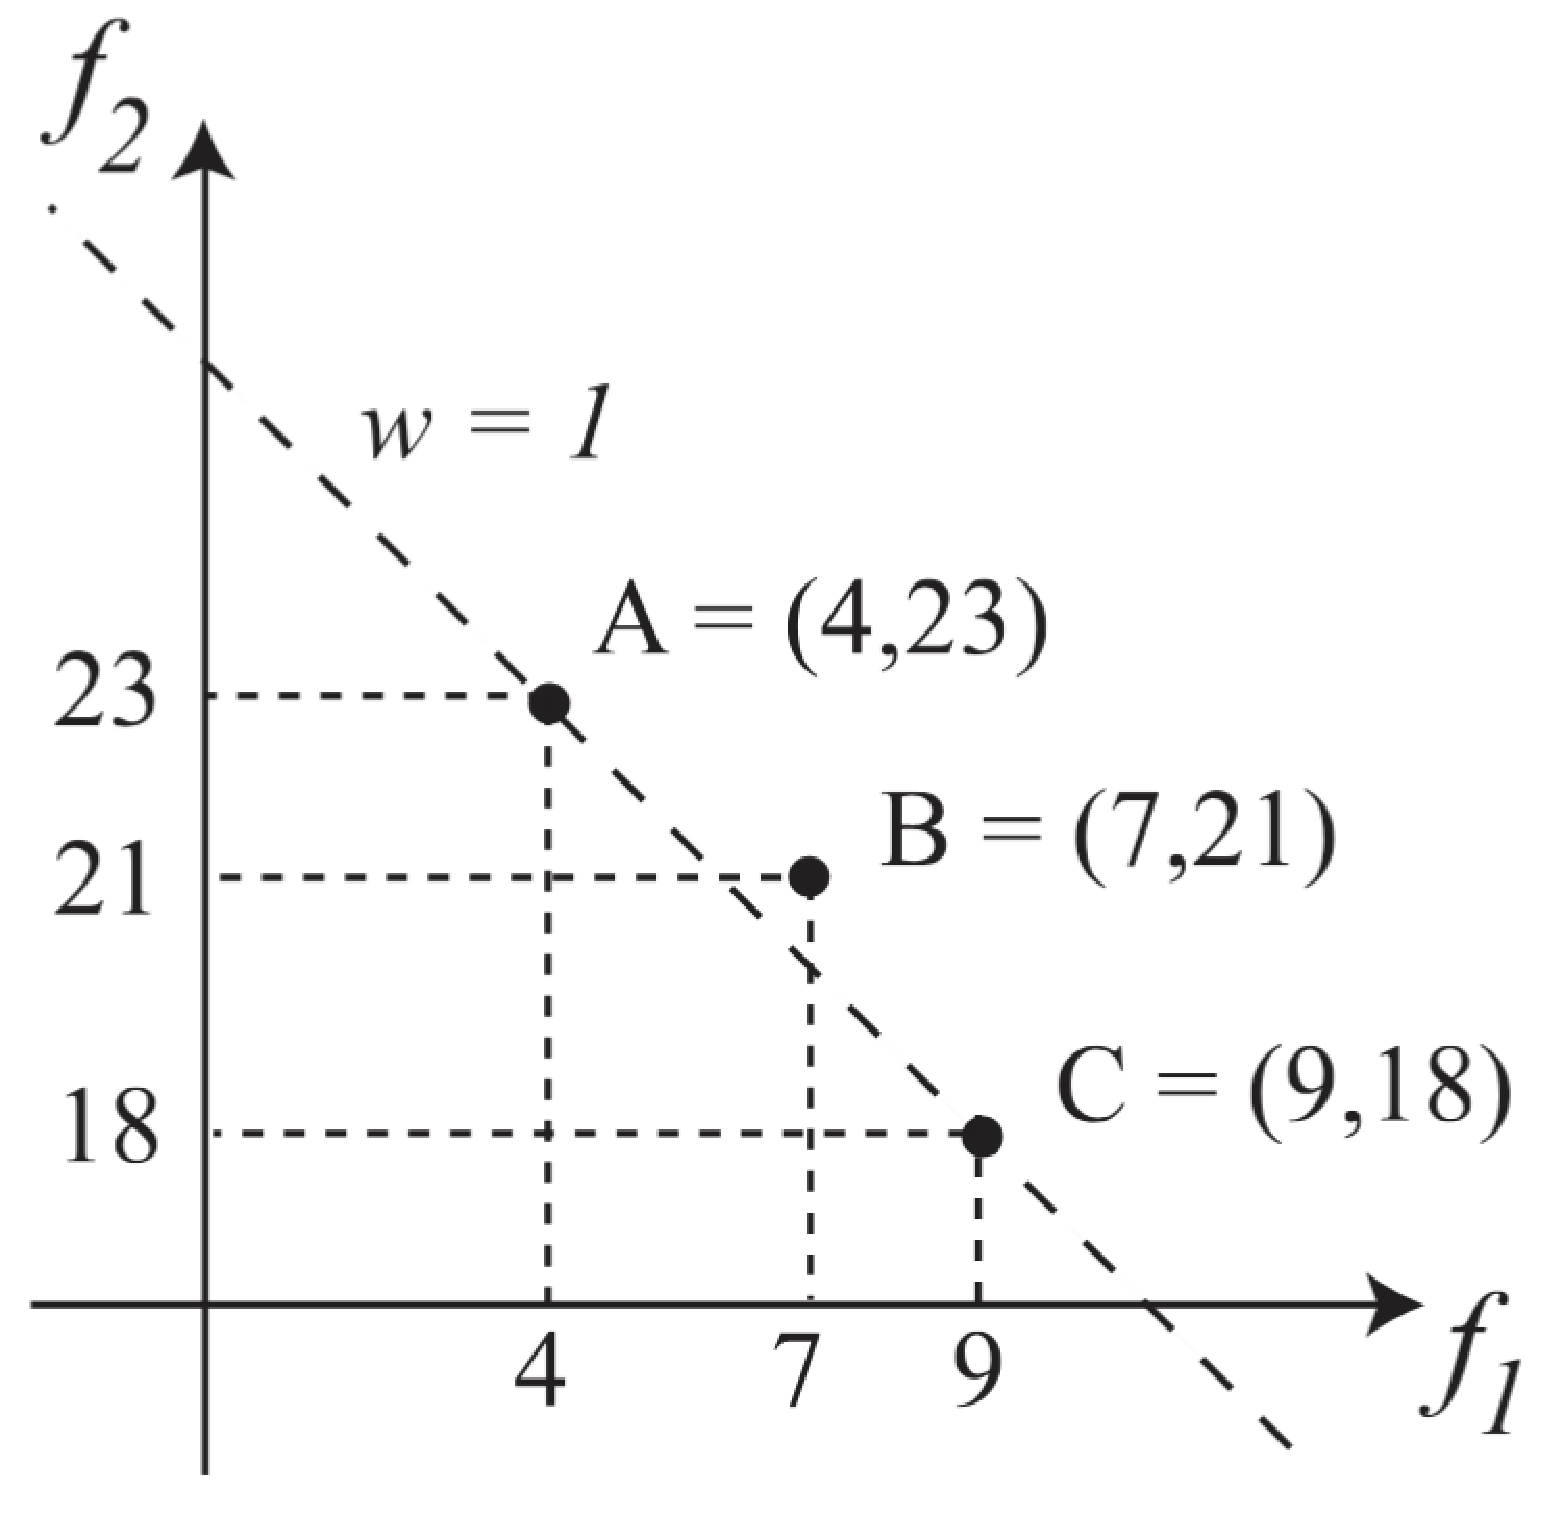
\includegraphics[width=0.4\columnwidth]{img/mcp/paretian/combex}
\end{center}

The weighted sum method solves the auxiliary parametric 
$$ \min z_w (x) = w f_1 (x) + (1 - w) f_2 (x) $$
combining the objectives $f_1$ and $f_2$ with the weights $w$ and $(1-w)$, where $w \in (0,1)$, and solving the minimum spanning tree problem for each value of $w$. The costs of the edges are:
\begin{itemize}
	\item $f(1,2) = w \cdot 1 + (1 - w) \cdot 13 = 13 - 12 w$
	
	\item $f(1,3) = w \cdot 3 + (1 - w) \cdot 10 = 10 - 7 w$
	
	\item $f(2,3) = w \cdot 6 + (1 - w) \cdot 8 = 8 - 2 w$
\end{itemize}

Making the problem
$$ \min z_w (x) = (13 - 12w) x_{12} + (1-7w)x_{13} + (8-2w)x_{23} $$
where $x$ is a spanning tree.

It's a minimum spanning tree with parametric costs on the edges $c_{ij} (w)$. The problem can be solved with Kruskal's algorithm: 
\begin{itemize}
	\item Sort the edges by increasing costs
	
	\item Include the edges that do not close loops
\end{itemize}

Let the weight vector $w$ vary in the weight space $W$, here $(0,1)$ and describe the costs $c_{ij} (w)$ of the three edges as a function of $w$.

\begin{center}
	\begin{tikzpicture}
		\begin{axis}[
			xlabel={$w$},
			grid=major,
			legend pos=south west,
			domain=0:1,
			samples=100,
			width=10cm,
			height=8cm
			]
			%Functions
			\addplot[blue, thick, name path=c12] {13-12*x};
			\addlegendentry{$c_{12}(w)$}
			\addplot[red, thick, name path=c13] {10-7*x};
			\addlegendentry{$c_{13}(w)$}
			\addplot[green, thick, name path=c23] {8-2*x};
			\addlegendentry{$c_{23}(w)$}
			
			% Find intersections
			\path[name intersections={of=c12 and c13, name=int1}];
			\path[name intersections={of=c12 and c23, name=int2}];  
			\path[name intersections={of=c13 and c23, name=int3}];
			% Mark the intersection points
			\fill[black] (int1-1) circle (2pt);
			\fill[black] (int2-1) circle (2pt);
			\fill[black] (int3-1) circle (2pt);
		\end{axis}
	\end{tikzpicture}
\end{center}

Find the regions in $W$ where each arc is the cheapest, second, etc. (intersections of the lines shown above)
$$ c_{23} (w) = c_{13} (w) \Leftrightarrow w = \frac{2}{5}$$
$$ c_{13} (w) = c_{12} (w) \Leftrightarrow w = \frac{3}{5}$$
$$ c_{23} (w) = c_{12} (w) \Leftrightarrow w = \frac{1}{2}$$

Apply Kruskal's algorithm to each region: 
\begin{itemize}
	\item If $w \in (0, 2/5]$, select $(2,3)$ and $(1,3)$ $ \implies T_3 $
	
	\item If $w \in [2/5, 3/5]$, select $(1,3)$, then
	\begin{itemize}
		\item if $w \in [2/5, 1/2]$, select $(2,3)$ $ \implies T_3 $
		
		\item if $w \in [1/2, 3/5]$, select $(1,2)$ $ \implies T_1 $
	\end{itemize}
	
	\item If $w \in [3/5, 1)$, select $(1,2)$ and $(1,3)$ $ \implies T_1 $
\end{itemize}

Solution $T_2$ is not found: it is unsupported ($\supp(T_2) = \emptyset$). Indeed, $T_2$ is nonoptimal for any convex combination of the indicators, even if it can be a good compromise.

\subsection{Advantages and Disadvantages}
\label{subsec:wsprocons}

The weighted-sum method has some strong advantages: 
\begin{enumerate}
	\item It can be applied to any problem, even the ones for which KKT conditions are useless (e.g., discrete problems)
	
	\item It's very intuitive, as often the decision-makers find it natural to combine the indicators by summing them, after choosing units of measure for which their numerical values are not too different
	
	\item It only requires to build an auxiliary object for the problem, keeping every other feature, and in particular the feasible region; quite often, a valid algorithm for the optimization of the single indicators is also valid for the optimization of the auxiliary objective
\end{enumerate}

At the same time it has strong disadvantages:
\begin{enumerate}
	\item It requires to consider all possible values of the weight vector $w$, which form a continuous infinite set; this requires a parametric solution, that is in general nontrivial, and for large-size problems can become intractable
	
	\item It requires to find all globally optimal solutions for each value of $w$ (one is not enough, contrary to Mathematical Programming)
	
	\item It does not provide the whole Paretian region $X^\circ$, but only the supported solutions, which could be a very restrictive underestimate \\
\end{enumerate}

\begin{theo}
	In a combinatorial problem, the number of nonsupported solutions can grow exponentially with respect to the number $n$ of decision variables; correspondingly, the weighted-sum method can provide a fraction of the Paretian region gradually converging to zero.
\end{theo}

To avoid the need for a parametric algorithm, it's possible to sample the set of weights $W$, but this further reduces the subset found and it can be inefficient (finding the same solution for several different weight vectors).

\subsubsection{Relations between the weighted-sum method and MAUT}

There are strong similarities between the weighted-sum method to determine the Paretian region and the MAUT (additive utility function and the auxiliary problem look similar), but the context is completely different:
\begin{enumerate}
	\item The weighted-sum method does not require complete preferences, nor mutual preferential independence or the corresponding trade-off condition, but only that the attributes be costs or benefits; partial order instead of a weak order
	
	\item The weighted-sum method does not require to determine a specific weight vector $w$, but it scans all possible vectors with strictly positive components; in MAUT the weights $w_l$ have a fixed value in $W$
	
	\item The weighted-sum method does not provide an "optimal" solution but a subset of the Paretian region 
	
	\item The weighted-sum method directly combines the attributes, without filtering them through utility functions suitably built so as to reflect the relative utilities associated to different values of an indicator; consequently, it cannot access the nonsupported solutions; on the contrary, suitable utility functions (suitably shaped indifference curves) allow the overall utility function to admit such solutions as optimal; MAUT can reach unsupported solutions
\end{enumerate}

\section{The $\epsilon$-constraint method}
\label{sec:epsconstraint}

The $\epsilon$-constraint method consists in replacing all indicators but one with constraints that require the solution to respect a quality threshold, and in solving the resulting auxiliary problem. The result is a necessary condition for a point to be globally Paretian (sufficient and necessary to be weakly Paretian).

The following theorem proves that all Paretian solutions are optimal points for a problem of this family, provided that the thresholds are suitably determined. \\

\begin{theo}
	If $x^\circ$ is a globally Paretian point for $f$ in $X$, $\epsilon_l = f_l (x^\circ)$ and $\ell \in P$, then $x^\circ$ is globally optimal for
	$$ \min z_\epsilon = f_\ell (x), \quad \forall x \in X $$
	$$ f_l \leq \epsilon_l, \quad l \in P \setminus \{\ell\}$$
\end{theo}
\begin{proof}
	The proof is by contradiction: suppose that $x^\circ$ is not globally optimal:
	$$ \exists x' \in X : \begin{cases}
		f_\ell (x') < f_\ell (x^\circ) \\
		f_l (x') \leq \epsilon_l = f_l (x^\circ) \ l \in P \setminus \{\ell\}
	\end{cases} \implies x' \prec x^\circ $$
	which goes against the paretianity of $x^\circ$. \\
\end{proof}

The auxiliary problem is parametric, to be solved for all vectors $\epsilon \in \R^{p-1}$ ($\infty^{p-1}$ values). Consequently, the solutions provided form a hypersurface of $\infty^{p-1}$ points.

\subsubsection{$\epsilon$-constraint and lexicographic preference}

The lexicographic method also focuses on a single indicator. \textit{Is there a relation with the $\epsilon$-constraint method?}

Not really, since lexicographic preference: 
\begin{itemize}
	\item Assumes a total order on impacts, not a partial order
	
	\item Discriminates optimal impacts based on the secondary indicator
	
	\item Doe snot impose aspiration levels $\epsilon_l$ on the secondary indicators
\end{itemize}

\subsection{Advantages and disadvantages}

The $\epsilon$-constraint method has some strong advantages:
\begin{enumerate}
	\item It can be applied to any problem, even the ones for which KKT conditions are useless (e.g., discrete problems)
	
	\item It's very intuitive, as often decision-makers find it natural to focus on a single indicator and to translate their preference into minimum satisfaction thresholds
	
	\item It provides an overestimate of the Paretian region that is often quite tight and can be easily refined applying again the method with a different choice of the main indicator
\end{enumerate}

At the same time, however, it has strong disadvantages: 
\begin{enumerate}
	\item It requires to consider all possible values of thresholds $\epsilon$, which form a continuous infinite set; this requires a parametric solution, that is in general nontrivial, and for large size problems can become intractable
	
	\item It requires to find all globally optimal solutions for each value of $\epsilon$ (one is not enough, contrary to Mathematical Programming)
	
	\item In combinatorial problems, while changing the objective function usually does not affect the computational complexity of the problem (the polynomial ones remain polynomial), introducing additional constraints nearly always increases the complexity (for example, a polynomial problem turns into an NP-complete one)
\end{enumerate}

% End L11, p203 notes, skipping excercises